\chapter{Numbering Systems}
How do we represent numbers? Based on how we represent numbers, certain operations
can be easier or harder. Today, we’ll consider two representations: decimal and
binary numbers. Decimal numbers --- decimal notation or base 10 --- are what we’re
all used to seeing in our daily lives. For example we could consider the string of
numerals:

$$ 19,874 $$

And we know this represents the value nineteen thousand eight hundred seventy four.
However, we could consider representing numbers differently. Depending on how we
represent numbers specific operations become easier or harder. Let’s go back to our
example and now we’ll multiply by 10.

\begin{align*}
19,874&\\
\underline{\times\hspace{6mm}10}&\\
198,740&\\
\end{align*}

We see it is very easy to find the answer --- we only need to add a 0 at the end
of our number.

Today we’ll see how to find the value of numbers represented in decimal and
binary notation. And how to convert between the two notations. We’ll start with
the decimal notation that we see in our everyday lives.

\section{Decimal Numbers}
When we see numbers in our daily lives there’s an implicit assumption that these
numbers are decimal numbers, whether this is a price, the temperature, or time.
We can be explicit about what representation we are using by subscripting our
numbers with the base.

$$ 19,874_{10} \hspace{7mm}\text{or}\hspace{7mm}  12.38_{10}$$

In this class and in real life, unless there is a subscript other than 10 below a number we consider all numbers to be
represented in base 10. So, for example, writing $19_{10}$ is the same as writing $19$. We'll use this base notation for representations other than decimal. 

\section{Radix Decomposition}
How do we actually go from numbers in base 10 to finding their value? We can break
down the number by each position, into what's called it's ``radix decomposition". Consider the radix decomposition of 19,874:

\begin{alignat*}{12}
& 19,874 &&=&& 1\times10,000 &&+&& 9\times1,000 &&+&& 8\times100  &&+&& 7\times10   &&+&& 4\times1    &\\
&             &&=&& 1\times10^4   &&+&& 9\times10^3  &&+&& 8\times10^2 &&+&& 7\times10^1 &&+&& 4\times10^0 &\\
\end{alignat*}

How do we know the value is nineteen thousand eight hundred seventy four? We can
break it down digit by digit and add together the values. We have 4 in the 1s (the
right-most position), 7 in the 10’s position, 8 in the hundreds position, 9 in the
thousands, and 1 in the ten-thousands position. Or in other words, at each
successive position we multiply the value of the digit at that position by the next
power of 10 to determine its value. This even works for non-whole numbers. Consider
the number:

\begin{alignat*}{10}
& 12.38 &&=&& 1\times10   &&+&& 2\times1    &&+&& 3/10           &&+&& 8/100            &\\
&            &&=&& 1\times10^1 &&+&& 2\times10^0 &&+&& 3\times10^{-1} &&+&& 8 \times 10^{-2} &\\
\end{alignat*}

We find 1 in the tens position, 2 in the ones position, 3 in the tenths position,
and 8 in the hundredths position. For non-whole numbers we treat every digit to the
right of the decimal (or radix) point exactly the same as we do for whole numbers.
Everything to the left of the radix point we successively divide by the next power
of ten. In practice, then, start at the decimal point. The number immediately to the left gets multiplied by $10^0$. The one to the left of that gets multiplied by $10^1$. We keep increasing the power of 10 by 1 as we move to the left. We then move from the decimal place to the right: multiply the first number to the right by $10^{-1}$, the second by $10^{-2}$, etc. We then add all these numbers together. 

\begin{example}
Write down the radix decomposition of the following decimal numbers: 
\begin{enumerate}
\item 3
\item 12
\item 10
\item 100
\item 2.22
\item 210.1
\end{enumerate}
\noindent \emph{Answer}:
\begin{enumerate}
\item $3\times10^0$
\item $1\times10^1+2\times10^0$
\item $1\times10^1+0\times10^0$
\item $1\times10^2+0\times10^1+0\times10^0$
\item $2\times10^0+2\times10^{-1}+2\times10^{-2}$
\item $2\times10^2+1\times10^1+0\times10^0+1\times10^{-1}$
\end{enumerate}
\end{example}

\ja{Is this going to be too fast, since some students will struggle with exponential notation?}

Now that we know how to determine the value of a decimal number, we
do the same for other number representations. 

\section{Binary Numbers}
What are binary numbers? They’re just another way to represent numbers; however,
instead of having ten digits (zero to nine) we have two bits (zero and one). Last
week, we learned about computer hardware. A computer’s primary purpose is to
compute; so we need to be able to store numbers on a computer’s hardware. Without
getting too technical, a computer represents numbers in a sequence of transistors,
each storing an electrical charge. These charges can be on (high voltage) or off
(low voltage) or somewhere in between. However, like with a light bulb that may burn
brighter or be dimmer based on the incoming charge, we only consider if the state
is on or off. 

Computers therefore represent numbers in binary. To better understand how
computers work, we’ll practice converting back and forth between the number representation system we're used to - decimal, or base 10 - and the number representation of computers - binary, or base 2. 

Importantly, when we convert between the representations, we're not changing the number itself, we're just writing it down in a different way. In the next section, we'll learn to ``read" binary!

%$$1_2 = 1_{10} \hspace{1cm} 11_2 = 3_{10} \hspace{1cm} 101_2 = 5_{10} \hspace{1cm} 110.01_2 = 6.25_{10}$$
%
%Here we see how we represent 1, 3, 5, and 6.25 in binary notation.

\section{Binary to Decimal Conversion}
We’ll now examine how to take binary numbers and convert them to their decimal notation. To do so, we will use the binary number's radix decomposition. The formula is to add together the number in each position multiplied by its corresponding power of 2 - the same process as for decimal numbers, but now with powers of 2 instead of powers of 10. 

Specifically, the number immediately to the left gets multiplied by $2^0$. The one to the left of that gets multiplied by $2^1$. We keep increasing the power of 2 by 1 as we move to the left. We then move from the decimal place to the right: multiply the first number to the right by $2^{-1}$, the second by $2^{-2}$, etc. We then add all these numbers together. Let's look at a few examples together:

\begin{alignat*}{12}
& 101_2 &&=&& 1\times2^2 &&+&& 0\times2^1 &&+&& 1\times2^0 & \\
&              &&=&& 4     &&+&& 0 &&+&& 1 & \\
&              &&=&& 5 &&  & \\
\end{alignat*}

Note that we can have fractional components of binary numbers the same way we do for decimal numbers. For example, 
\begin{alignat*}{12}
& 1.11_2 &&=&& 1\times2^0 &&+&& 1\times2^{-1} &&+&& 1\times2^{-2} & \\
&              &&=&& 1 &&+&& 0.5 &&+&& 0.25 & \\
&              &&=&& 1.75 &&  & \\
\end{alignat*}

\begin{example}
The numbers below are represented in base 2, or binary. Write down their base 10, or decimal, representation. 
\begin{enumerate}
\item $1_{2}$
\item $10_{2}$
\item $111_{2}$
\item $11.1_{2}$
\item $11.01_{2}$
\item $100011_{2}$
\end{enumerate}
\noindent \emph{Answer}:
\begin{enumerate}
\item $1\times2^0=\mathbf{1}$
\item $1\times2^1+0\times2^0=\mathbf{2}$
\item $1\times2^2+1\times2^1+1\times2^0=\mathbf{7}$
\item $1\times2^1+1\times2^0+1\times2^{-1}=\mathbf{3.5}$
\item $1\times2^1+1\times2^0+0\times2^{-1}+1\times2^{-2}=\mathbf{3.25}$
\item $1\times2^5+0\times2^4+0\times2^3+0\times2^2+1\times2^1+1\times2^0=\mathbf{35}$
\end{enumerate}
\end{example}

\begin{figure}
	\centering
	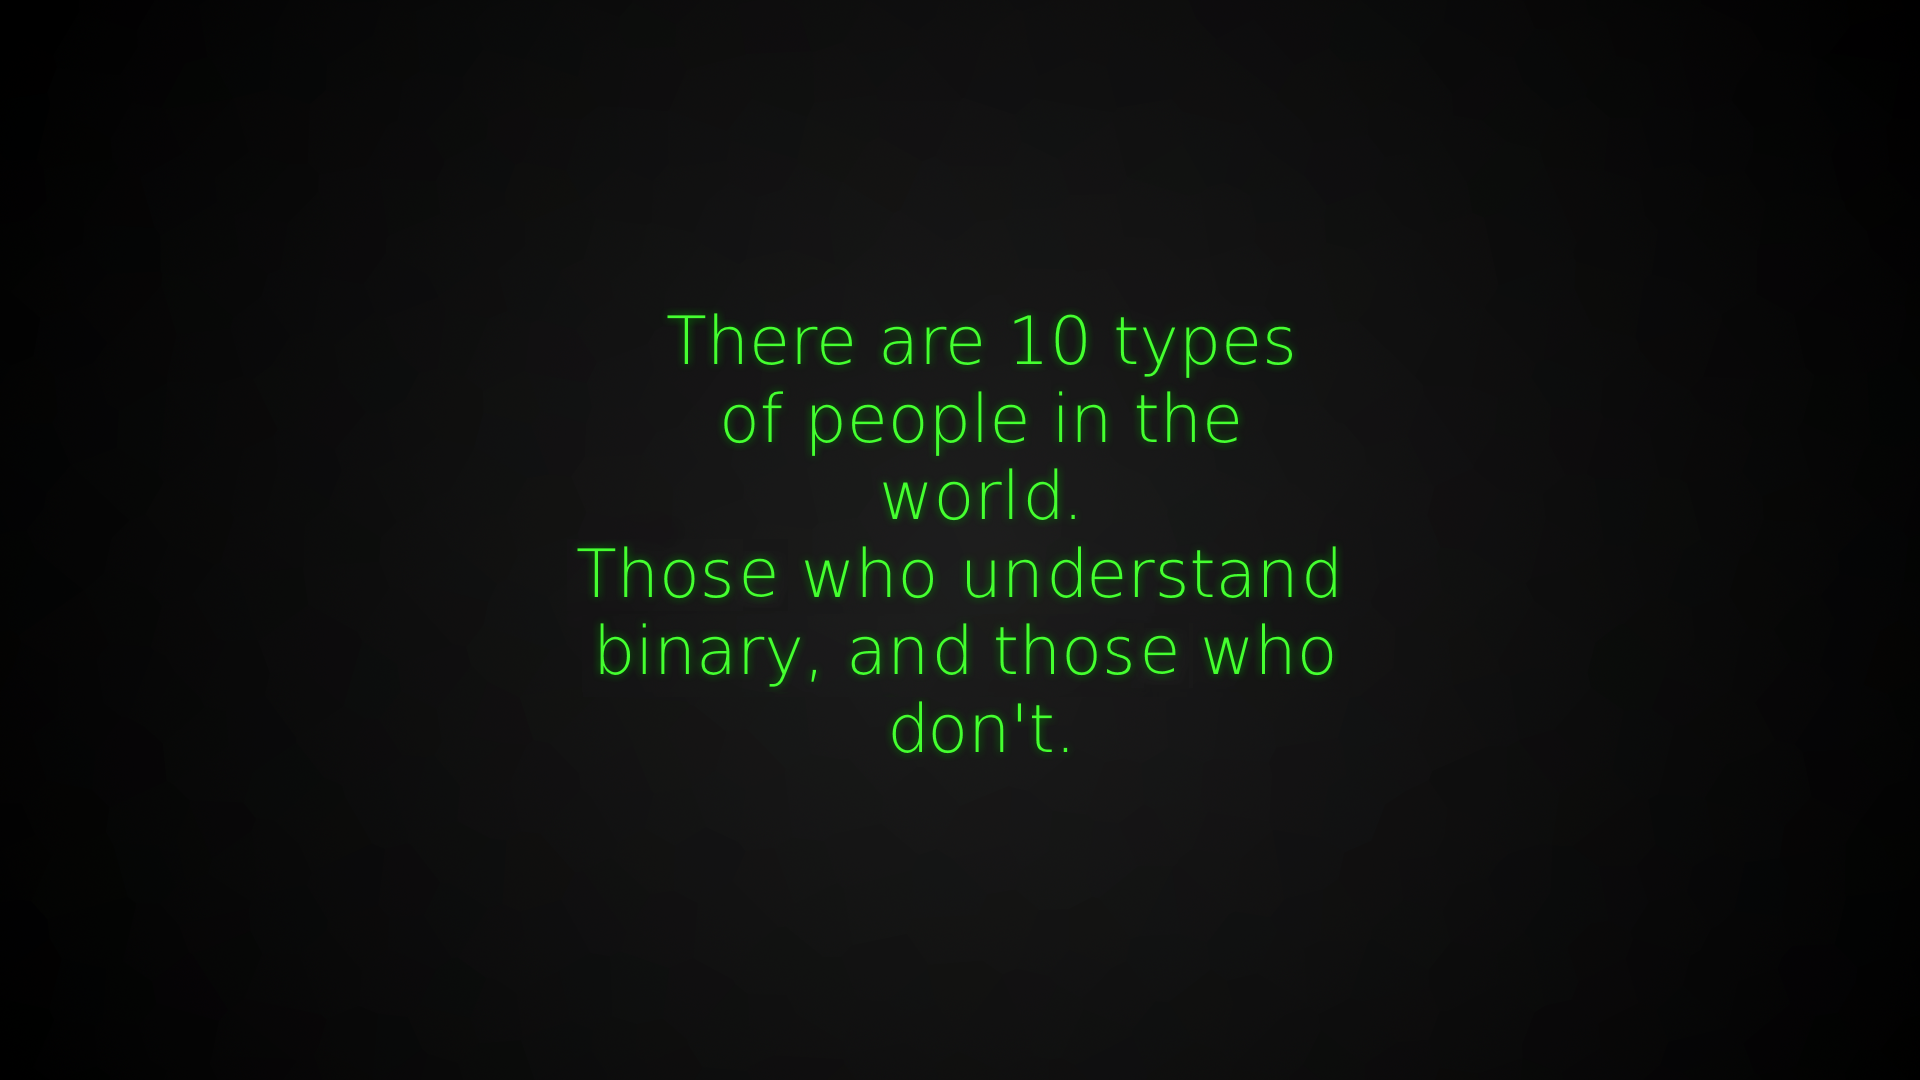
\includegraphics[width=0.85\textwidth]{images/binary_joke}
	% https://imgur.com/gallery/QkR1X
	\caption{A popular joke among nerds.}
	\label{fig:binary_joke}
\end{figure}

\section{Decimal to Binary Conversion}
Now, let’s look at the opposite conversion, converting decimal numbers to
binary. This will use successive division and subtraction as opposed to
addition and multiplication. We will divide by two. Then, if the
remainder is non-zero, we’ll keep a 1 at the current position. Otherwise, we'll write down a 0. We’ll
continue until we can no longer divide by two. We will use a table for this, where the first column is the number at the current step in the process; the second column is that number divided by 2 (excluding the remainder); and the third column is a 1 if there was a remainder and 0 otherwise. Here's the process for writing the binary representation of 33: 

\begin{center}
\begin{tabular}{|c|c|c|}
\hline
\textbf{Initial Value} & \textbf{Divided by 2} & \textbf{Remainder} \\
\hline
  4 &   2 & 0 \\
  2 &   1 & 0 \\
  1 &   0 & 1 \\
\hline
\end{tabular}
\end{center}

$$4 = 100_2$$

To walk through the process, 4 divided by 2 is 2. There is no remainder, so we put 2 in the second column and a 0 in the third column. We then moved 2 down to the first column in the next row. We divided 2 by 2 and got 1, which has no remainder so we wrote 0 in the last column. We brought down the 1, divided by 2 and got 0.5 (i.e. ``0 with a remainder of one"). So we wrote 0 in the second column, but for the remainder we put 1 in the third column. We then simply wrote down the string of numbers in the third column starting at the bottom and going up. 

Let's walk through one more example together: what is the binary representation of 13? 

\begin{center}
\begin{tabular}{|c|c|c|}
\hline
\textbf{Initial Value} & \textbf{Divided by 2} & \textbf{Remainder} \\
\hline
  13 &   6 & 1 \\
  6 &   3 & 0 \\
  3 &   1 & 1 \\
  1 &   0 & 1 \\
\hline
\end{tabular}
\end{center}

$$13 = 1101_2$$

To walk through the process, 13 divided by 2 is 6.5 (i.e. ``6 with a remainder of one"). There is a remainder, so we put 6 in the second column and a 1 in the third column. We then moved 6 down to the first column in the next row. We divided 6 by 2 and got 3, which has no remainder so we wrote 0 in the last column. We brought down the 3, divided by 2, and got 1.5 (i.e. ``1 with a remainder of one"). So we wrote a 1 in the second column and 1 in the third column. We brought down the 1, divided by 2 and got 0.5 (i.e. ``0 with a remainder of one"). So we wrote 0 in the second column and 1 in the third column. We then simply wrote down the string of numbers in the third column starting at the bottom and going up. 

It is also possible to convert decimal numbers that have a fractional part using this same method, but it can get challenging so we won't do it in this course. 

\begin{example}
The numbers below are represented in base 10, or decimal. Write down their base 2, or binary, representation. 
\begin{enumerate}
\item $1$
\item $2$
\item $5$
\item $10$
\item $20$
\item 
\end{enumerate}
\noindent \emph{Answer}:
\begin{enumerate}
\item $1_{2}$
\item $10_{2}$
\item $101_{2}$
\item $1010_{2}$
\item $10100_{2}$
\end{enumerate}
\end{example}

\section{Binary Addition}
Just as we perform addition with decimal numbers, we can perform addition with
binary numbers. The process is exactly the same, except we work with bits (1s and 0s) instead of
digits (0 through 9). Let’s start by looking at addition and multiplication in decimal.

\begin{align*}
15&\\
\underline{+\hspace{1mm}6}&\\
21&\\
\end{align*}

To get there, we looked at the rightmost numbers and added them to get 11 (i.e. ``10 remainder 1"). So we wrote down the remainder of 1 below the black line, and put a one on top of the line to the left. We then added 1 to 1 on the next line to get 2. Here's another example: 

\begin{align*}
26&\\
\underline{+\hspace{1mm}17}&\\
30&\\
\end{align*}

Here we looked to the rightmost numbers, adding 6 to 7 to get 13 (i.e. ``10 remainder 3"). We wrote down the remainder of 3 below the line and carried a 1 (for the 10) to the top of the next column. We then added 1, 2, and 3 in that column to get 6. Let's try one more:

\begin{align*}
55&\\
\underline{+\hspace{1mm}60}&\\
115&\\
\end{align*}

We went to the rightmost numbers and added them: 5 and 0 give 5 (i.e. ``0 remainder 5"). So we wrote down the remainder of 5 below the line and didn't need to carry anything. We moved left and added 5 to 6 to give 11 (i.e. ``10 remainder 1"). So we wrote down a 1 and moved a 1 to the next column (which was empty). We then simply brought down the 1. 

The process is exactly the same for binary numbers! Instead of have 10 with remainders, though, we will think about 2 with remainders. Let's jump straight into an example to clarify this, where we'll add $111_{2}$ (7 in decimal representation) to $11_{2}$ (3 in decimal representation). If all goes well, we should get $1010_{2}$, since that is 10 in decimal representation. 

\begin{align*}
111_{2}&\\
\underline{+\hspace{1mm}11_{2}}&\\
1010_2&\\
\end{align*}

Here we looked at the rightmost column and added 1 and 1 together to get 2 (i.e. ``2 remainder 0"). We wrote down the remainder of 0 below the line and carried a 1 (for the 2) to the top of the next column. We then had to add 1, 1, and 1, which gives us 3 (i.e. ``2 remainder 1"). So we wrote a 1 below the line (for the remainder of 1) and carried a 1 (for the 2). Finally, we added 1, 1, and 0 to get 2 (i.e. ``2 remainder 0"). So we wrote down 0 below the line and carried a 1 (for the 2). We then simply brought down the 1. 

Let's look at one more example together: 

\begin{align*}
111_{2}&\\
\underline{+\hspace{1mm}111_{2}}&\\
1110_2&\\
\end{align*}

We start on the right and add 1 and 1 to get 2 (i.e. ``2 remainder 0"). So we write 0 below the line and carry a 1. We then add 1, 1, and 1 to get 3 (i.e. ``2 remainder 1"). So we write down a 1 and carry a 1. We then add 1, 1, and 1 to get 3 (i.e. ``2 remainder 1"). We wrote down a 1 and carried a 1 (for the 2). We then simply brought down the 1. 

\begin{example}
Add the following binary numbers. Give your answer in binary representation. 
\begin{enumerate}
\item $1_2+1_2$
\item $11_2+1_2$
\item $101_2+111_2$
\item $1110_2+1_2$
\end{enumerate}
\noindent \emph{Answer}:
\begin{enumerate}
\item $10_2$
\item $100_2$
\item $1100_2$
\item $1111_{2}$
\end{enumerate}
\end{example}

Subtraction, multiplication, and division of binary numbers also involves the same process as decimal numbers. However, we won't go over these in this course. 

%\noindent%
%\begin{minipage}{.5\linewidth}
%\begin{align*}
%10110101_2&\\
%\underline{+\hspace{1mm}1010110_2}&\\
%100001011_2&\\
%\end{align*}
%\end{minipage}%
%\begin{minipage}{.5\linewidth}
%\begin{align*}
%110101_2&\\
%\underline{\times\hspace{3mm}1101_2}&\\
%110101_2&\\
%11010100_2&\\
%\underline{+\hspace{1mm}110101000_2}&\\
%1010110001_2&\\
%\end{align*}
%\end{minipage}

%Here we see how to add the binary representations of 181 and 86 and get 267 as the
%result. We also see how to do long form multiplication of 53 and 13 to get 689. You’ll
%notice this is exactly the same as for decimal numbers but we force ourselves to only
%work with bits, carrying the one to the next place when necessary. Both subtraction
%and division work similarly.

\section{Bit-wise Operators}

Now we’ll turn our attention to three important arithmetic operations on binary numbers:
\textbf{and}, \textbf{or}, and \textbf{exclusive or} (\textbf{xor}). These are
called ``bit-wise operations" as they apply to each bit place, one at a time. We therefore can simply line up two binary numbers, padding with 0s on the left of the shorter binary number if they are different lengths (which doesn't change its value). We'll see an example of the process later, but first let's understand what the operators do to an individual set of 2 bits.  

When looking at two binary numbers, \textbf{and} is an operation that gives 1 if both bits are 1, and 0 otherwise (i.e. answers ``the first \textbf{and} second bit are both 1?"). The \textbf{or} is an operation that gives 1 if either bit (or both bits) is 1 (i.e. answers ``is either/or bit 1?"). Finally, the ``exclusive or", or \textbf{xor}, is an operation that gives 1 if either bit (but \textit{not} both) is 1 (i.e. answers ``is exclusively one of the bits 1?"). The following table lists out the result of each operation on every combination of 0 and 1. 

\begin{center}
\begin{tabular}{|c|c|c|c|c|}
\hline
$a$ & $b$ & $a$ \textbf{and} $b$ & $a$ \textbf{or} $b$ & $a$ \textbf{xor} $b$ \\
\hline
0   &  0  &  0  &  0  &  0  \\ 
0   &  1  &  0  &  1  &  1  \\
1   &  0  &  0  &  1  &  1  \\
1   &  1  &  1  &  1  &  0  \\
\hline
\end{tabular}
\end{center}

Now that we know how to operate on any two bits, we can simply line up any two binary numbers (with left-zero padding as necessary) and use the operator on each set of bits. Here are a few examples: 

To do $111_2\textbf{and}110_2$:
\begin{align*}
111_2 &\\
\underline{\textbf{and}\hspace{2mm}110_2}&\\
110_2 &\\
\end{align*}

In this example, the two numbers are the same length so we don't need to pad any zeros. Starting with the rightmost bits, we have $1\mathbf{and}0$ which is $0$. Moving to the left, we have $1\mathbf{and}1$, which is 1. Moving to the left again, we have $1\mathbf{and}1$, which is 1

Now let's do $101_2\mathbf{or}11_2$:
\begin{align*}
101_2 &\\
\underline{\mathbf{or}\hspace{4mm}011_2}&\\
111_2&\\
\end{align*}

In this case, since $11_2$ is shorter than $101_2$, we needed to pad the 11 with a single 0 on the left so it was also three bits long. We then did bit-wise comparison: from right to left we saw $1\mathbf{or}1$ is $1$, $0\mathbf{or}1$ is $1$, and $1\mathbf{or}0$ is $1$. 

Now let's do $111_2\mathbf{xor}1_2$:
\begin{align*}
101_2 &\\
\underline{\mathbf{xor}\hspace{4mm}001_2}&\\
100_2 &\\
\end{align*}

Since $111_2$ has three bits and $1_2$ only one, we pad two zeros on $1_2$ to get $001_2$. We then go from right to left with the \textbf{xor} operation, getting $1\textbf{xor}1=0$, $0\textbf{xor}0=0$, and $1\textbf{xor}0=1$.

Finally, try $111_2\mathbf{and}1_2$:
\begin{align*}
101_2 &\\
\underline{\mathbf{and}\hspace{4mm}001_2}&\\
1_2 &\\
\end{align*}

As in the previous example, since $111_2$ has three bits and $1_2$ only one, we pad two zeros on $1_2$ to get $001_2$. We go from right to left with \textbf{and}, getting $1\textbf{and}1=1$, $0\textbf{and}0=0$, and $1\textbf{and}0=0$. So our results is $001_2$. However, since left-padded 0s don't change the number this is the same as $1_2$. 

\begin{example}
Perform the following binary operations. Give your answer in binary representation. 
\begin{enumerate}
\item $1_2 \textbf{xor}1000_2$
\item $10_2 \textbf{or} 10_2$
\item $1111_2 \textbf{and} 1011_2$
\item $1111_2 \textbf{or} 1011_2$
\end{enumerate}
\noindent \emph{Answer}:
\begin{enumerate}
\item $1001_2$
\item $10_2$
\item $1011_2$
\item $1111_{2}$
\end{enumerate}
\end{example}

\exercisesection

\begin{exercise}
Write the radix decomposition for each of these decimal numbers. For example, 1.2's radix expansion is $1\times10^0 + 2\times10^{-1}$
\begin{enumerate}
\item 193 
\item 5.2
\item 1,984
\item 7.39
\end{enumerate}
\end{exercise}

\begin{exercise}
Write out the radix decomposition for each of these binary numbers. For example, $1.1_2$'s radix expansion is $1\times2^0 + 1\times2^{-1}$. 
\begin{enumerate}
\item $11_2$
\item $10.1_2$
\item $1.01_2$
\item $111_2$
\end{enumerate}
\end{exercise}

\begin{exercise}
Write out the decimal form of the following binary numbers. For example, $1.1_2$'s in decimal form is $1.5$. These are the same numbers as in the previous exercise, so feel free to use the radix decompositions you already wrote down. 
\begin{enumerate}
\item $11_2$
\item $10.1_2$
\item $1.01_2$
\item $111_2$
\end{enumerate}
\end{exercise}

\begin{exercise}
Write out the binary form of the following decimal numbers. 
\begin{enumerate}
\item 6
\item 15
\item 22
\item 80
\end{enumerate}
\end{exercise}

\begin{exercise}
Add the following binary numbers. Write the answer in binary form. 
\begin{enumerate}
\item $1_2 + 0_2$
\item $111_2+1_2$
\item $111_2+111_2$
\item $101_2+100_2$
\end{enumerate}
\end{exercise}

\begin{exercise}
Evaluate the following bit-wise operations. Write the answer in binary form. 
\begin{enumerate}
\item $1_2 \mathbf{and} 0_2$
\item $111_2 \mathbf{or} 1_2$
\item $111_2 \mathbf{xor} 111_2$
\item $101_2 \mathbf{and} 100_2$
\end{enumerate}
\end{exercise}